\section{Distributed Storage}

How can we store a huge amount of large files across many nodes in a network? Which components in the network change over time? Can we do something better than a global index (what file is stored on which node)?


\subsection{Consistent Hashing}

We might want to use some sort of hashing, e.g. consistent hashing (we already have seen this concepts in other lectures).\medskip

\begin{algorithm}[H]
\caption{Consistent Hashing}
	Hash the unique file name of each file $x$ with a known set of hash functions $h_i(x) \mapsto [0, 1)$, for $i = 1,...,k$ \\
	Hash the unique name (e.g. IP address and port number) of each node with the same hash function $h(u) \mapsto [0, 1)$ \\
	Store a copy of movie $x$ on node $u$ if $h(x) \approx h(u)$, for any $i$. More formally, store movie $x$ on node $u$ if :
$$|h_i(x) -  h_(u)| \min_v \{|h_i(x) -  h_(v)|\}, \text{ for any } i$$	
\end{algorithm}
\medskip

In expectation, each node in this algorithm stores $km/n$ files, where $k$ is the number of hash functions, $m$ the number of different files and $n$ the number of nodes. \medskip

We can also choose to use pointers, then we can store the files on any node we like (e.g. a data centre) and let the weaker nodes simply return the forward pointer to the actual location. For better load balancing, we might want to hash multiple times. \medskip

In this chapter, we consider nodes with high churn: nodes are very unreliable and may only be available for a short amount of time. In this scenario, as hundreds of nodes will change every second, no single node can have an accurate picture of all the other nodes in the system. It is impossible to have a consistent view at any time. \medskip

A node will have information about its neighbors (a small subset of all nodes). Thus, it does not directly know which node is responsible for what file. Instead, it asks its neighbor who recursively asks its neighbor, too. Thus, the nodes form a virtual network (an overlay network).


\subsection{Hypercubic Networks}

Our virtual network should have the following properties:
\begin{itemize}
	\item The network should be more or less \textbf{homogeneous}, i.e. no node plays a dominant role and there is no single point of failure.
	\item The nodes should have \textbf{IDs}. all the IDs should span the universe $[0,1)$.
	\item Every node should have a \textbf{small degree}. This allows a node to maintain a persistent connection with each neighbor, allowing us to deal with churn.
	\item The network should have a \textbf{small diameter} and routing should be easy. If a node doesn’t have the required information itself, it should know which neighbor it must ask. Within a few hops, we should find the node containing the correct information.
\end{itemize}

One possible network topology that can be used are trees. Routing is very easy, but basic trees are not homogeneous: the root is a bottleneck. Using \textbf{fat trees} where every edge connecting $v$ to its parent $u$ has a capacity that is proportional to the number of leaves in the subtree of $v$.
\begin{center}
	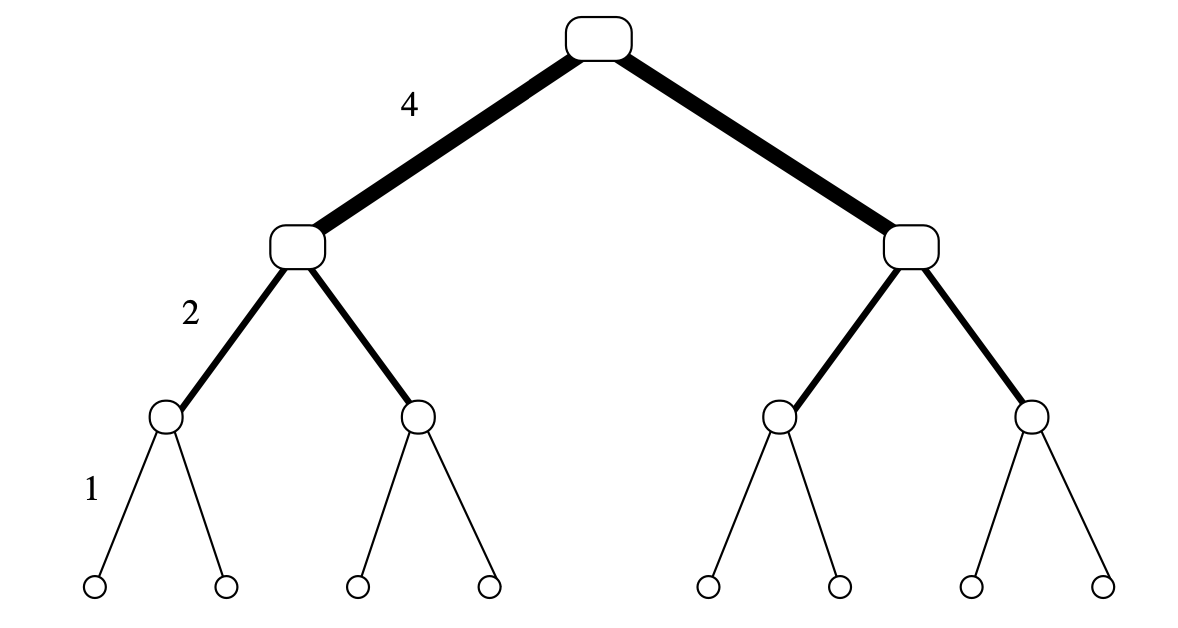
\includegraphics[width=\linewidth]{fat_tree.png}
\end{center}

Another topology are tori and meshes: Let $m,d \in \N$, the $(m,d)$-mesh $M$ is a graph with node set $V = [m]^d$ (vectors of length $d$ of numbers $\{1,...,n\}$) and edge set
$$E = \left \{   \{(a_1,...,a_d), (b_1,...,b_d) \; | \; a_i, b_i \in [m], \sum_{i=1}^d |a_i, b_i| = 1 \} \right \}$$

The $(m,d)$-torus $T(m,d)$ is a graph that consists of an $(m,d)$-mesh and additionally wrap-around edges from nodes $(a_1, ..., a_{i-1}, m - 1, a_{i+1}, ..., a_d) $ to nodes $(a_1, ..., a_{i-1}, 0, a_{i+1}, ..., a_d)$ for all $i \in \{1, ...,d\}$ and all $a_j \in [m]$ with $j \neq i$. $M(m,1)$ is a path, $T(m,1)$ a cycle and $M(2,d) = T(2,d)$ a $d$-dimensional hypercube.

\begin{center}
	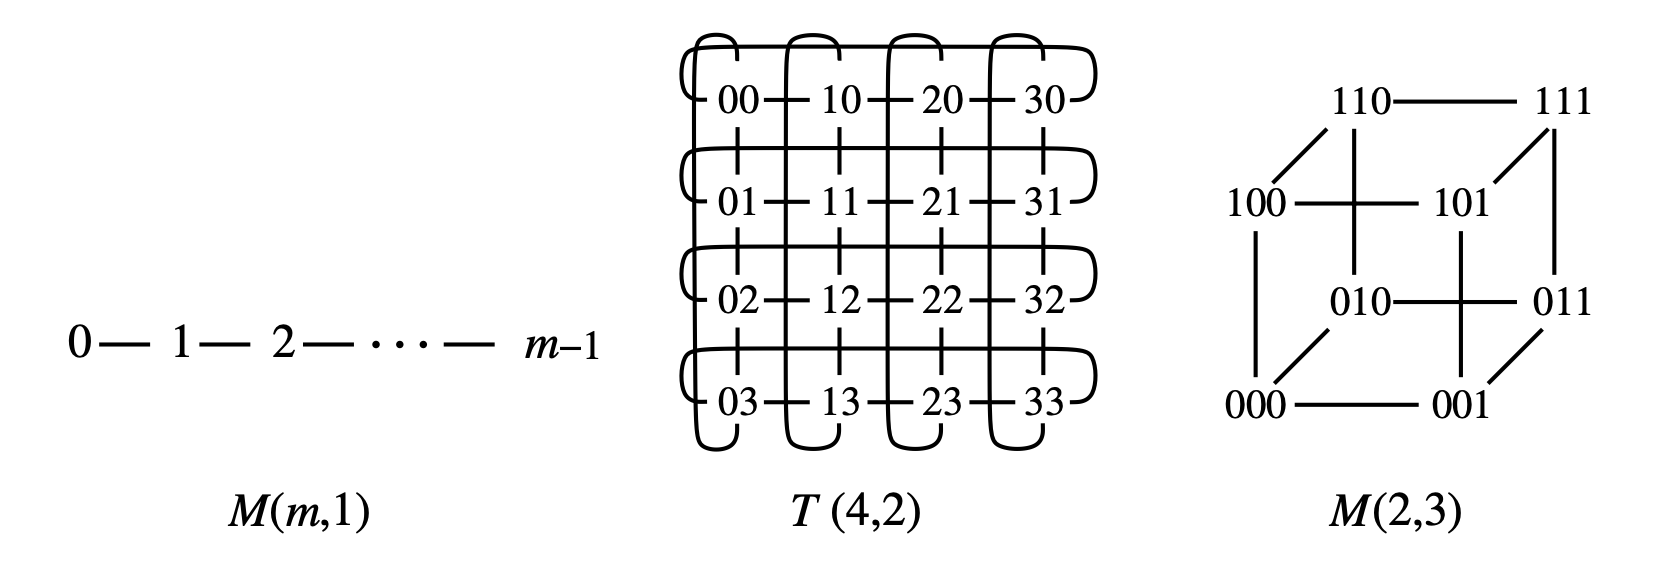
\includegraphics[width=\linewidth]{mesh.png}
\end{center}

Routing on a mesh, torus, or hypercube is trivial. On a $d$-dimensional hypercube, to get from a source bitstring $s$ to a target bitstring $t$ one only needs to fix each "wrong" bit, one at a time. There are $k!$ routes with $k$ hops. \medskip

We need to map the $d$-bit IDs to the universe $[0, 1)$. We can do so, by interpreting the bitstring $b = b_1 ... b_d$ as the number $\sum_{i=1}^d 2^{-i} b_i = (0.b_1 ... b_d)_2$ in binary. \medskip

There are many topologies that are similar to hypercubes, e.g. the Chord architecture. The hypercube connects every node with an ID in $[0,1)$ with every node in exactly distance $2^{-i}$. Chord instead connects nodes with approximately distance $2^{-i}$. Many of the following examples are also derivatives of hypercubes.

\subsubsection{Butterfly}

The $d$-dimensional butterfly $BF(d)$ is a graph with node set $V = [d+1] \times [2]^d$ and edge set $E = E_1 \cup E_2$ where:
$$E_1 = \{\{ (i, \alpha), (i+1, \alpha)\} \; | \; i \in [d], \alpha \in [2]^d\}$$
$$E_2 = \{\{ (i, \alpha), (i+1, \beta)\} \; | \; i \in [d], \alpha, \beta \in [2]^d, \alpha \oplus \beta = 2^i \}$$

The node set $\{(i, \alpha) \; | \; \alpha \in [2]^d\}$ forms the level $i$ of the butterfly. 
\begin{center}
	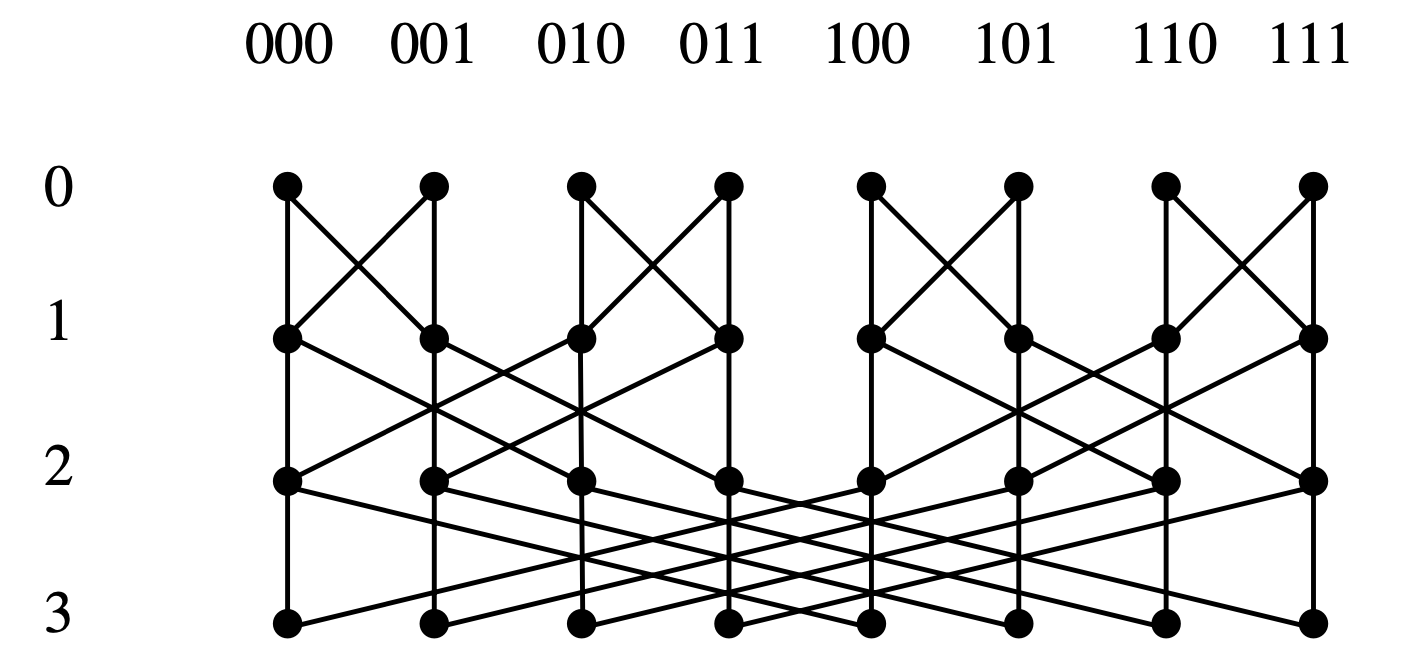
\includegraphics[width=0.8\linewidth]{butterfly.png}
\end{center}

The $d$-dimensional wrap-around butterfly $W - BF(d)$ is defined by taking the $BF(d)$ and having $(d, \alpha) = (0, \alpha)$ for all $\alpha$. \medskip

Butterflies have the advantage of a constant node degree over hypercubes, whereas hypercubes feature more fault-tolerant routing.

\subsubsection{Cube-Connected-Cycles}

The cube-connected-cycles network $CCC(d)$ is a graph with node set $V = \{ (a,p) \; | \; a \in [2]^d, p \in [d] \} $ and edge set \smallskip

$E = \{\{ (a,p), (a, p+1 \mod d) \} \; | \; \alpha \in [2]^d, p \in [d]\} \cup \{\{(a,p), (b,p)\} \; | \; a,b \in [2]^d, p \in [d], |a-b| = 2^p \}$ \smallskip

$CCC(3)$ results from the hypercube by replacing the corners by cycles. We can represent it in 2 different ways:
\begin{center}
	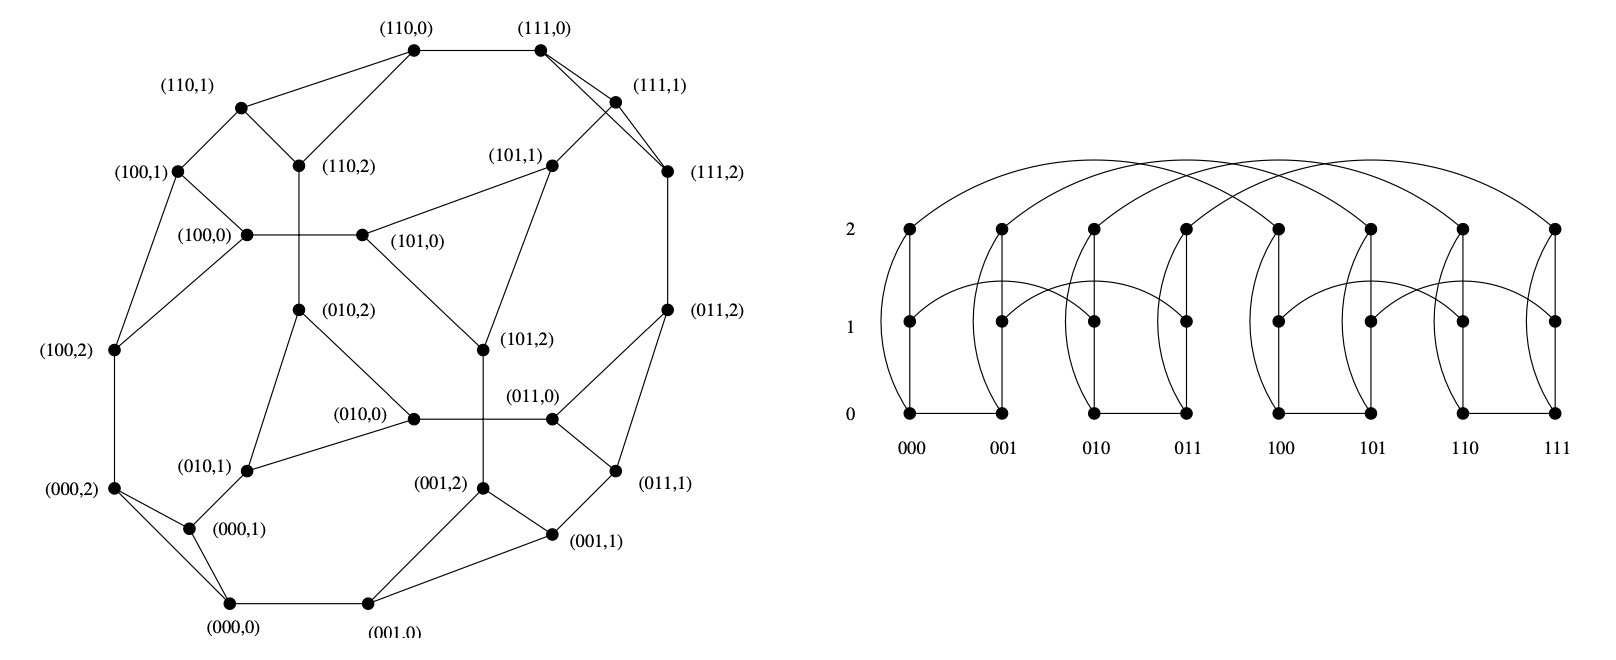
\includegraphics[width=\linewidth]{ccc.png}
\end{center}

\subsubsection{Shuffle-Exchange and DeBrujin}

The shuffle-exchange and the DeBruijn network are other ways of transforming the hypercubic interconnection structure into a constant degree network. \medskip

\textbf{Shuffle-Exchange}
\begin{center}
	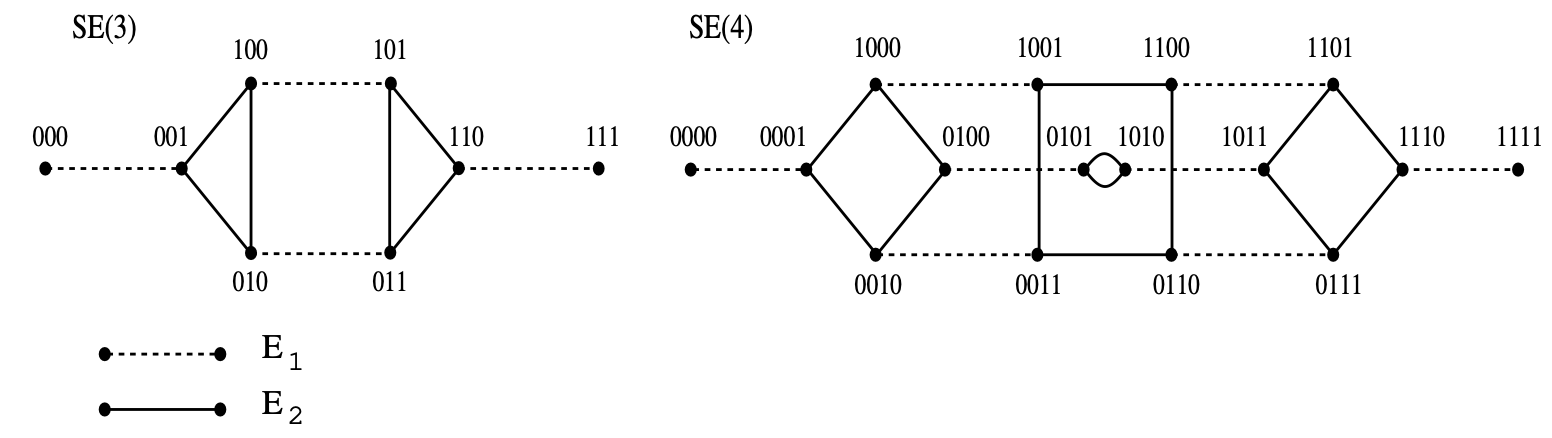
\includegraphics[width=0.9\linewidth]{shuffel_network.png}
\end{center}

\textbf{DeBrujin}
\begin{center}
	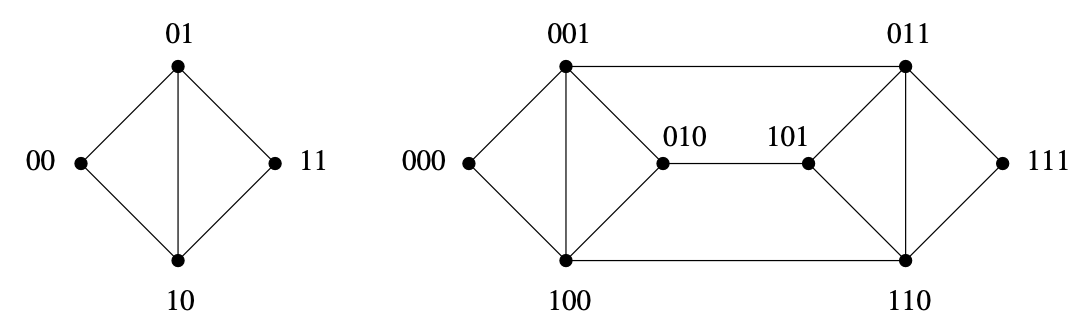
\includegraphics[width=0.9\linewidth]{debruijn.png}
\end{center}

\subsubsection{Skip List}

The skip list is an ordinary ordered linked list of objects, augmented with additional forward links. The ordinary linked list is the level 0 of the skip list. In addition, every object is promoted to level 1 with probability 1/2. As for level 0, all level 1 objects are connected by a linked list. In general, every object on level $i$ is promoted to the next level with probability 1/2. A special start-object points to the smallest/first object on each level. \medskip

Search, insert, and delete can be implemented in $\mathcal{O}(\log n)$ expected time in a skip list. There are obvious variants of the skip list, e.g., the skip graph. \medskip

Back to more general properties of hypercubic networks. In general, there is a trade o↵ between degree and diameter. Every graph of maximum degree $d > 2$ and size $n$ must have a diameter of at least $\lceil \log n / \log (d-1) \rceil -2$. In other words, constant-degree hypercubic networks feature an asymptotically optimal diameter $D$. Other hypercubic graphs manage to have a different tradeoff between node degree $d$ and diameter $D$.


\subsection{DHT and Churn}

A distributed hash table (DHT) is a distributed data structure that implements a distributed storage. A DHT should support at least (i) a search (for a key) and (ii) an insert (key, object) operation, possibly also (iii) a delete (key) operation. \medskip

A DHT can be implemented as a hypercubic overlay network with nodes having identifiers such that they span the ID space $[0, 1)$. We assume that a joining node knows a node which already belongs to the system. One way to do this is using some authority for a list of IP addresses of nodes that might be in the system. \medskip

To analyze this network against adversary, we assume that an adversary can remove and add a bounded number of nodes. It can choose which nodes to crash/join. Also, the adversary does not have to wait until the system is recovered before it crashes the next bash of nodes. \medskip

Our system is never fully repaired, but always fully functional. An adversary can add/remove at most $\mathcal O (\log n)$ nodes in a constant time interval. This covers repeatedly taking nodes down in a DDoS attack. Also we assume no message delays which can be achieved using time synchronization.\medskip

\begin{algorithm}[H]
\caption{DHT}
	Given: a globally known set of hash functions $h_i$ and a hypercube network \\
	Each hypercube virtual node ("hypernode") consist of $\Theta(\log n)$ nodes \\
	Nodes have connections to all other nodes of their hypernode and to nodes of their neighboring hypernodes \\
	Because of churn, some of the nodes have to change to another hypernode such that up to constant factors, all hypernodes own the same number of nodes at all times \\
	If the total number of nodes $n$ grows or shrinks above or below a certain threshold, the dimension of the hypercube is increased or decreased by one, respectively
\end{algorithm}
\medskip

Thus, each node has $\Theta(\log^2 n)$ neighbors. One can achieve $\Theta (\log n)$ with some additional effort. \medskip

The balancing of nodes can be seen as a dynamic token distribution problem on the hypercube. Each hypernode has a certain number of tokens and the goal is to distribute them along the edges s.t. all hypernodes end up with roughly the same number of tokens. \medskip

Using DHT with churn, we have a fully scalable, efficient distributed storage system which tolerates $\mathcal O(\log n)$ worse case joins and/or crashes per constant time interval. Nodes have $\mathcal O (\log n)$ overlay neighbors and search/insert take time $\mathcal O (\log n)$.


